\chapter{From a push-based to an open, pull-based development model}

\label{chap:pull-based-development}

\section{Introduction}

Ever since they were invented, version control systems (VCS) have been invaluable tools for effective software development and maintenance~\cite{spinellis2005vcs}.

However, for distributed collaboration around source code, and more specifically for open source development, the first generation of VCS (CVCS, i.e. centralized version control systems) were not really effective because only developers with commit-access could benefit from them~\cite{de2009software,rodriguez2012distributed}.
So the introduction of distributed version control systems (DVCS), such as git~\cite{torvalds2005git}, has been a great step forward for collaborative and open source development.
They alleviate having to worry about who has commit-access~\cite{torvalds2007git}, and make it possible to review changes, including large changes, \emph{before} they are pushed to the main development branch.\footnote{
	The practice of code review is still possible, in any VCS, \emph{after} the changes are pushed~\cite[Chapter 2]{fogel2005producing}, but conducting systematic \emph{a posteriori} code reviews requires a much stronger culture.
	And some CVCS, such as SVN~\cite{svn} have sufficiently good branching support to allow developer teams to adopt \emph{a priori} code reviews.
}

Finally, social coding platforms (such as GitHub~\cite{github}) have simplified the submission and code review process.
The general consolidation of open source development around GitHub (and competitors such as GitLab~\cite{gitlab}) has helped to create a unified contribution workflow~\cite{opensourceguide}, which can benefit smaller projects without formalized contribution guidelines, and contributors, who know approximately what to expect when approaching a new project.

Empirical software engineering research has also benefited from the sudden availability of very large datasets of public and consistently-organized software repositories.
This has allowed researchers to study various questions associated with the pull-based development model~\cite{cosentino2017systematic}.

\begin{description}
	\item[Pull-based development] is a development model based on a DVCS where anyone can clone a repository, make changes, push to a branch on their own fork (public development copy) of the project, then request the project owners to integrate (pull) their changes to the official repository.
	It is defined by opposition to the traditional \emph{push-based} development model, where developers with commit rights push their changes to a central repository, and contributors without commit rights must resort to formatted patches submitted via e-mail or a bug tracker.
	\item[Social coding] is an approach to software development that puts the focus on collaboration, in particular through online discussion around code, and across projects (such as when developers from related projects investigate a bug together~\cite{ma2017developers}). Social coding is grounded in pull-based development on coding platforms, like GitHub, where specific review tools make it possible to discuss around code, and where it is easy to cross-reference issues and pull requests across different projects. The ``social coding'' motto was part of GitHub's logo from 2009 to 2011.\footnote{
		From the beginning of the archival of GitHub.com by the Wayback Machine~\cite{waybackmachine} in May 2008 (\url{http://web.archive.org/web/20080514210148/http://github.com/}), to January 2009 (\url{http://web.archive.org/web/20090115203245/http://github.com/}), the motto that appeared in the logo was ``social code hosting''. It was simplified down to ``social coding'' in February 2009 (\url{http://web.archive.org/web/20090201192503/http://github.com/}), and the logo was kept unchanged until December 2011 (\url{http://web.archive.org/web/20111214080929/https://github.com/}), when a new version was introduced (\url{http://web.archive.org/web/20111220204645/https://github.com/}).
	}
\end{description}

In this chapter, I present a historical overview of the use of VCS, and the move from a push-based to a pull-based development model in the Coq project, then I present four challenges associated with the new model.

The first challenge is how to onboard new contributors.
This was the initial motivation for using pull requests in the Coq project, but this alone is not sufficient to attract new contributors~\cite{dias2016does}, and I explain the steps we have taken to make it easier for newcomers to join the project.
The literature on newcomer onboarding is extensive~\cite{STEINMACHER201567}, and most of these steps are straightforward applications of standard recommendations, so this is more of an experience report than a novel contribution.

The second challenge is to improve quality through the use of pull requests.
This was the second motivation for the definitive switch to a pull-based model.
I explain how we introduced labels to help reviewers, and how I organized them in categories, which allowed to create even more of them.
I show that this phenomenon is not unique to the Coq project, and would deserve further investigations.
Then, I present the use of pull request templates, and show how this caused an increase in the quality of pull requests.
To my knowledge, this is the first analysis to show the impact of the introduction of pull request templates.

The third challenge is how to use continuous integration (CI) to test for compatibility with external reverse dependencies.
I present the innovative model that we introduced, and how it helped developers better apply our compatibility policy, and assess which breaking changes are acceptable.

The fourth and last challenge is how to distribute the review workload.
I explain how we managed to switch from a model with a single integrator, to a team of 25 integrators (larger than the ``core team'' which comprises 10 developers), in part by relying on the recently introduced \verb|CODEOWNERS| GitHub feature~\cite{github_code_owners}.
While the Coq project is not the first one to use this feature, this is, to my knowledge, the first academic report about it.

\section{Related work}

\subsection{GitHub studies}

Since GitHub took off as the central platform for collaborative, pull-based development, many academic papers have been published studying various aspects of the practice of development on GitHub.

In the first paper to study social coding, Dabbish \emph{et al.}~\cite{dabbish2012social} interviewed GitHub users and observed their use of the website. They determined that transparency in GitHub and visibility of others' actions allowed increased collaboration and learning, for instance between project owners and their users.

Gousios \emph{et al.} studied pull-based development from the integrator's~\cite{gousios2015work}, and the contributor's~\cite{gousios2016work} perspective. They found that most projects use pull requests to sollicit external contributions, but that many also use it for reviewing all code changes, and some require multiple reviews before integrating a change. Quality is the top priority during the review process, and it is evaluated through perception and tools (but few tools are used beyond continuous integration). Integrators face challenges such as maintaining quality, especially when pull requests are too large to review properly, and rejecting contributions without alienating contributors. The challenges faced by the contributors are the unresponsiveness of maintainers, the lack of documentation or guidelines to understand the code base, of proper testing infrastructure, of a project's roadmap, and of a list of issues labeled by difficulty level.

In 2017, Cosentino \emph{et al.} produced a survey of the literature on GitHub~\cite{cosentino2017systematic}. They identified 80 relevant papers (most from 2013--2016, five from 2012, and one from 2010). About 70\% exclusively rely on mining software repositories, while the rest use survey and interviews, possibly in addition to mining software repositories. The works that they cite found among other things that very few GitHub projects attract most code contributions and most issues, that very few developers are responsible for most code contributions, and that drive-by contributions are very common. Numerous studies (15 papers) analyzed the socio-technical predictors associated with pull request acceptance / rejection, and the time it takes to evaluate a pull request. Among the uncovered predictors, it was observed that larger pull requests take longer to review, and are more likely to get rejected, and that pull requests sent to large and mature projects are also more likely to get rejected.

\subsection{Switch to git and GitHub}

While a great number of papers studied the characteristics of GitHub's development model, very few studied the impact of switching to this platform for an older project having been previously developed in a push-based forge, without as many social features. Dias \emph{et al.} did such kind of study on six major open source projects~\cite{dias2016does}. They observed that a switch to GitHub is not always immediately followed by an increased number of contributions or contributors, and that other factors, like having clear contribution guidelines, and being ready to review pull requests, are equally important.
Roveda \emph{et al.}~\cite{roveda2017does} evaluated if the code quality of projects migrating to GitHub is affected, and did not detect any such effect.

Other researchers studied the switch of projects to DVCS.
De Alwis and Sillito~\cite{de2009software} surveyed developers to understand the perceived impact of moving from centralized to decentralized VCS: the move is decided because of anticipated benefits (among them the openness to external contributors), but the switch incurs challenges in the migration process (in particular, developers are very concerned to preserve the full history of the project) and some features are lost in the new tool (in particular, the chronologically ordered revision numbers).
Muşlu \emph{et al.}~\cite{mucslu2014transition} performed a similar study based on interviews and a survey. They identified expectations and barriers and provided recommendations to developers wanting to conduct such a migration.
Brindescu \emph{et al.}~\cite{brindescu2014centralized} analyzed the impact of using decentralized or centralized VCS through data mining and a survey. They found most notably that the type of VCS is associated with commits of different sizes.

\section{Historical overview: towards pull requests}

\label{sec:towards-pull-requests}

From at least 1991, Coq was developed using version control systems.\footnote{
	Source: \url{https://github.com/coq/coq/blob/5f7c88d/dev/doc/archive/versions-history.tex\#L111}.
}
In 1999, the repository that is still in use today (after a conversion to git~\cite{torvalds2005git}) was started using SVN~\cite{svn}, by copying and refactoring code originating from the previous CVS~\cite{cvs} archive. This repository now comprises about 30,000 commits.

A mirror of the SVN repository was created in February 2011 at \url{https://github.com/coq/coq}. This repository received a first pull request a few months later,\footnote{
	\url{https://github.com/coq/coq/pull/1}
} that was acknowledged with some delay with the message ``This is just a mirror [...]. None of the primary developers of coq watch this repo. If you want to get this merged, you shuold [\emph{sic}] post it to http://coq.inria.fr/bugs/''.
The second pull request was received a year later,\footnote{
	\url{https://github.com/coq/coq/pull/2}
} acknowledged by a Coq developer, and merged as an SVN revision with a delay of almost one year.

The development repository was switched to git in November 2013~\cite{letouzey_svn_to_git}, but GitHub remained just a mirror, and the development style was still push-based, with numerous developers having got commit-access over the years.\footnote{ \label{footnote:forge}
	The page at \url{https://gforge.inria.fr/projects/coq} lists 54 project members, one of them (G Serpyc) being a bot account.
}
From then on, pull requests were one of the officially listed ways of proposing patches (formatted patches submitted via the bug tracker were also still accepted), and the activity on GitHub was notified on the Coq developers' mailing list.
In the following months, dozens of pull requests were opened by just one contributor (and a few more by three other contributors), most of them getting integrated without any comment, a few already giving rise to reviews or comments by other external contributors.\footnote{
	See \url{https://github.com/coq/coq/pull/31} and \url{https://github.com/coq/coq/pull/33}.
}
In September 2014, a pull request was used by a core developer for the first time in order to get a review (proofreading a documentation submission).

The core developers started to seriously advertise GitHub pull requests as a way to integrate external contributions during the first Coq Implementors Workshop in 2015.\footnote{
	This first workshop was actually called ``Coq coding sprint'', and its purpose was to onboard external contributors by having them meet core developers that could answer their questions. It has been held every year since then, for three years under the name ``Coq Implementors Workshop'', and in 2019 under the name ``Coq Users and Developers Workshop''.
	\label{footnote:coq_implementors_workshop}
}
A year later, during the 8.6 release process, they started regularly using pull requests to submit their own changes.
Finally, after the adoption of CI (see Section~\ref{sec:ci}) developers stopped pushing changes without going through a pull request.
More than 3,000 pull requests have been merged since the beginning.

Figure~\ref{fig:github_contributors} shows the growth of the number of contributors who opened pull requests on the GitHub repository. We can notice that a few core contributors opened many pull requests, and many other contributors opened a few pull requests.
Out of ten contributors who opened more than 100 pull requests, five were core developers in the previous, push-based model. The other five gained push-access when the merging process was distributed (see Section~\ref{sec:distributed-merging}).

However, this figure does not really allow the viewer to distinguish between drive-by contributors~\cite{pham2013building} and regular, but infrequent contributors. Figure~\ref{fig:github_contributors2} shows all the pull requests that have been opened by each contributor.
On this figure, we can more clearly distinguish between the contributors who open just one pull request (about 40\% of all the contributors), the ones who open a few pull requests and then disappear, and the ones who stay but contribute infrequently.

These figures were created using the data from the analysis in Section~\ref{sec:rdd1} (cf. the corresponding notebook~\cite{zimmermann2019contributors}).
The list of developers who had push-access on the repository before the switch to a pull-based development model was extracted from the previous project page, mentioned in Footnote~\ref{footnote:forge}, and manually matched to GitHub accounts.
Two developers who gained push-access after having first contributed to Coq through pull requests are not marked as having had push-access before.
Conversely, the developer who opened the very first pull request (that was completely ignored) gained push-access shortly after. Therefore, this first pull request has been removed from the dataset, and the developer has been classified as having had push-access.

\begin{figure}
	\begin{center}
		\includegraphics{../notebooks/github-contributors/github_contributors.png}
		\caption{
			Contributors to the Coq GitHub repository.
			Each dot represents a contributor.
			Its horizontal position corresponds to the date the contributor opened their first pull request.
			Its vertical position represents a counter of the number of contributors so far.
			The area of the dot is proportional to the number of pull requests that the contributor has opened since then.
			Dark indigo dots represent contributors who already had push access \emph{before} opening their first pull request.
		}
		\label{fig:github_contributors}
	\end{center}
\end{figure}

\begin{figure}
	\begin{center}
		\includegraphics{../notebooks/github-contributors/github_contributors2.png}
		\caption{
			Pull requests on the Coq GitHub repository grouped by author.
			All the pull requests opened by the same contributor are grouped at the same vertical position (and their horizontal position denotes the date when they were opened).
			Contributors are ordered by when they opened their first pull request.
		}
		\label{fig:github_contributors2}
	\end{center}
\end{figure}

\begin{figure}
	\begin{center}
		\includegraphics{../notebooks/bug-tracker/pull_requests_nb.png}
		\caption{
			Total number of pull requests opened per day by main developers and by other contributors.
			Each point represents an average over a four-week period.
			The distinction between the two categories is based on the number of commits, as explained in Section~\ref{sec:variables}.
		}
		\label{fig:pull_request_nb}
	\end{center}
\end{figure}

Figure~\ref{fig:pull_request_nb} shows the evolution of the number of pull requests opened per day by main developers and by other contributors.
It was generated by reusing the analysis pipeline of the bug tracker switch (see Chapter~\ref{chap:bug-tracker}).

\section{How to onboard new contributors?}

\label{sec:newcomers}

Core developers are sufficiently many to address by themselves all the issues (bugs and feature requests) that would be worth addressing.
Furthermore, core developers frequently leave the project, or become less active, because their focus has changed, and it is important to get new active contributors that can take their place.
Finally, the landscape of proof assistants is evolving rapidly, and Coq has both well-established (Isabelle/HOL), and new (the Lean prover) competitors (that are free software as well), thus evolving too slowly could lead Coq to become less successful, as users turn to more modern / shiny solutions.
For all these reasons, it seems important to onboard new contributors that can become regular, active developers.

While drive-by contributions do not generally represent a large proportion of the code changes~\cite{robles2009evolution}, they are also essential to get small fixes, in particular documentation fixes. Indeed, the ones that are most likely to read, and thus discover problems with the documentation, are the users, rather than the developers who feel that they already know the documentation well.

Some actions can be implemented that specifically encourage drive-by contributions, such as a visible ``Edit on GitHub'' button on each documentation page, or asking to users reporting a bug and proposing a solution whether they would be willing to open a pull request. Some other actions can be taken specifically to retain new contributors, such as providing feedback quickly, and showing appreciation (for instance the reaction system that GitHub introduced in 2016~\cite{github_reactions} provides an easy, and non-intrusive%
\footnote{
	Leaving a reaction on an issue, pull request, or comment does not generate any notification that could lead someone to interrupt their work.
	Reactions are displayed visibly, but do not take any additional space in a discussion thread.
}
way of showing appreciation, that can help newcomers feel welcome%
\footnote{
	For some anecdotal evidence, see: \url{https://gitter.im/coq/coq?at=5b3758513d8f71623d51075b}.
}%
).

Code documentation, and contributing guidelines, are essential to new contributors, as was highlighted by Gousios \emph{et al.}~\cite{gousios2016work}.
This was frequently reminded by the new contributors themselves, and their pressure and contributions have been an efficient way of improving such documentation.
In particular, a good way of getting better internal documentation that will help the next contributors is often to encourage the newcomers who ask questions to write down and share the answers they get.%
\footnote{
	Cf. in particular \url{https://github.com/coq/coq/pull/961}, where a contributor introduced the first version of the contributing guide, after getting annoyed with something he did not understand, and having discussed it on our Gitter~\cite{gitter} chat; \url{https://github.com/coq/coq/pull/6557}, where a contributor introduced the test-suite documentation, after asking some questions about it, and being encouraged by myself to start such a document; \url{https://github.com/coq/coq/pull/7942}, where a contributor introduced a beginners' guide and an index of the developer documentation, after I encouraged him to do so on Gitter.
}

The contributing guide~\cite{coq_contributing_guide}, in particular, is the central piece of documentation aimed at explaining the contribution process to newcomers, and serves as a reference to regular contributors.
Its first version was created by an external contributor.
I have recently refactored, rewritten, and expanded it, so that it can serve as an exhaustive reference of the state of our current development processes (contributing guides are rarely exhaustive descriptions of the development processes according to Elazhary \emph{et al.}~\cite{elazhary2019not}).
It is structured in a way that follows the same path as new contributors, from contributions to the ecosystem, to bug reporting and small fixes, to larger contributions and involvement in the merging process~\cite{jensen2007role, nakakoji2002evolution, ye2003toward}.

\subsection{Future work}

So far, efforts to bring Coq developers and users closer, such as the creation of the Coq Implementors Workshop (cf. Footnote~\ref{footnote:coq_implementors_workshop}) have been quite successful to transform users into regular contributors.
As we will see in Chapter~\ref{chap:bug-tracker}, the switch of bug tracker from Bugzilla to GitHub, has also resulted in more external contributors participating in the discussions on issues.
In the future, I would like to try to bring development discussions closer to where the users might find them, thanks to the Discourse forum that was launched recently.

Discourse~\cite{discourse} is a new generation, open source, forum software, with a good mailing-list mode.
It has been adopted by a great number of open source projects, such as Atom \url{https://discuss.atom.io/}, Docker \url{https://forums.docker.com/}, Elm \url{https://discourse.elm-lang.org/}, Ember.js \url{https://discuss.emberjs.com/}, OCaml \url{https://discuss.ocaml.org/}, and Rust \url{https://users.rust-lang.org/}.

A user who had used the OCaml instance suggested that we create one for Coq, which I did in the beginning of 2019, after Discourse announced free hosting for open source projects~\cite{discourse2018free}, and after having got support from the rest of the development team.

One of the advantages of such a forum over mailing lists,%
\footnote{
	Other advantages being that it is easier to browse and search past questions and answers, and that users do not need to subscribe to a list in order to ask a question.
}
even for users that wish to use it in mailing-list mode, is that it is possible to mute all activity belonging to some categories.
This opens the door to creating categories for a subset of users, such as non-English categories.
It also makes it possible to move activity from several mailing lists, such as a developers' mailing list and a users' mailing list to distinct categories of a single forum.
This is something that Python did by gathering many mailing lists (committers', developers', users' mailing lists) into a single forum \url{https://discuss.python.org/}.

In their case, they decided to restrict who can post (but not who can read) the committers' category.
In the case of the Coq Discourse forum \url{https://coq.discourse.group/}, the development category is open to all, but has not been used much so far.

I hope to convince the development team to close the developers' mailing list in favor of this forum, as a way to bring development discussions closer to where users can see them.
Given the number of communities already using Discourse actively, there might be enough data already available to analyze the effect of such a switch, similarly to what Squire~\cite{squire2015should} and Vasilescu \emph{et al.}~\cite{vasilescu2014social} did about Stack Overflow.

\section{How to improve quality through the use of pull requests?}

\label{sec:quality}

Because they provide an opportunity for code review, the use of pull requests is largely considered to be associated with a higher level of quality of integrated changes~\cite{katilius2019quality}.
However, such an effect on quality is not easily measured, and also not automatic as it strongly depends on the quality of the review process itself.
Instead of addressing the general question of code quality in this section, I address a more specific question: how to ensure that pull request authors include changes to the documentation, the changelog, and the test-suite, in their pull requests, when such changes are needed.

While it should normally be the role of reviewers to ensure that such changes have been included, it is not always easy for them to remember that they have to check this.
To make their job easier, we have introduced two changes: ``needs'' labels, and pull request templates.

\subsection{Label categories, the ``needs'' labels}

\label{sec:labels}

Labels are quite useful to quickly mark different type of pull requests (or issues), and their current status.
Previous work~\cite{cabot2015exploring} has shown that few projects use labels on their issues (3.25\% of non-fork repositories hosted on GitHub), but this result is not surprising given that other studies have highlighted the fact that most GitHub projects are single-person projects~\cite{kalliamvakou2016depth}, and rarely use issues at all~\cite{bissyande2013got}. Projects where more people are involved are also associated with a higher number of labels.

When a project starts to use more and more labels, the costs may start outweighing the benefits, because participants are not necessarily aware of all the labels that are available, or what they mean. To alleviate this effect, some projects have adopted strategies based on gathering labels in consistent sub-groups. Given that GitHub sorts labels alphabetically, this strategy is particularly efficient when label sub-groups are identified by a common prefix.

After the use of labels in the Coq project had grown to a level where this problem was starting to show up, I introduced two categories (``needs:'' and ``kind:'') and distributed all the preexisting labels between the two.
The switch to the GitHub issue tracker, and the migration of preexisting issues (see Chapter~\ref{chap:bug-tracker}) led to the addition of new categories (``part:'', ``resolved:'', ``platform:''). 
Overall, the lesson of introducing these categories is that it has allowed the number of labels to grow much further, from 11 labels before the introduction of the categories to 89 today.\footnote{
	8 labels were created following the introduction of the categories; 32 labels were created during the bug tracker migration; 38 labels have been created since then.
}

The ``needs:'' category is especially useful for pull request reviewers as a way of reminding what needs to be done before a pull request can be merged. The absence of labels of this category is even checked automatically by the script that is used to merge pull requests (see Section~\ref{sec:distributed-merging}). This category currently comprises 21 labels, notably a ``needs: documentation'' label, a ``needs: changelog entry'' label (initially ``needs: CHANGES'', before the redesign of the changelog presented in Section~\ref{sec:release-notes}), and a ``needs: test-suite update'' label.

These categories (the ``needs:'' category in particular) were inspired by similar categories in the nixpkgs project\footnote{
	See \url{https://github.com/NixOS/nixpkgs/labels}.
} and have since then inspired the Math-Comp project.\footnote{
	See \url{https://github.com/math-comp/math-comp/labels}.
}
Even though label archeology is difficult on GitHub, because GitHub does not keep the history of label renamings and deletions, nor the name of their creators, we can still extract from the GitHub GraphQL API the list of all labels in a project, in the order they were created, their creation date, and the date of their last update. I identified that way that the current naming pattern of labels in the nixpkgs project dates back from November 21--22, 2015, and was introduced by Nicolas Pierron. After I wrote to him, he gave me some pointers,\footnote{
	E-mail thread in which the introduction of categories was discussed: \url{https://nixos.org/nix-dev/2015-November/018714.html}.
	This was not the first time such an idea was proposed: \url{https://nixos.org/nix-dev/2015-March/016549.html}.
} and told me that the inspiration to create categories was Rust.
Rust categories are a single letter followed by a dash\footnote{
	See \url{https://github.com/rust-lang/rust/labels}.
}
but Nicolas thought it was important that label categories be understandable by humans (labels can now carry a description but this feature was only added in 2018~\cite{github_label_descriptions}), so he introduced longer prefix categories, with an initial number to sort them.
The introduction of categories allowed the number of labels of the project to grow from 27 to 114 today.\footnote{
	6 labels were created automatically when the repository was created on June 4th, 2012;
	21 labels were created between July 20th, 2012 and November 16th, 2015;
	14 additional labels were created on November 21--22, 2015 by Nicolas Pierron when he introduced the categories;
	20 labels were created in just the following year;
	53 labels have been created since then.
}

A further cursory look at the labels of a hundred popular projects leads me to believe that not all popular projects use many labels, but among those that do, most use a similar pattern, where a prefix of the name indicates a category (the separator ``:'' is quite frequent, but we can also find the separators ``/'' and ``-'').
In particular, the Angular.js project has used similar categories, including the ``needs:'' category, since August 2013.\footnote{
	See \url{https://github.com/angular/angular.js/labels} and \url{https://github.com/angular/angular.js/blob/04a570d/TRIAGING.md}.
}
Again a similar growth in the number of labels can be observed.\footnote{
	14 labels were created between the project's creation date in January 2010 and February 2013; 10 labels were created during the month of August 2013 when the categories were introduced; 48 labels were created in just the following year; and 25 since then.
}
Overall, it would seem that the creation of categories fosters the growth of the number of labels (as we have observed in the Coq, nixpkgs, and Angular.js projects), but this would have to be confirmed through a more in-depth study.

\subsection{Pull request templates with checklists}

\label{sec:template}

Labels are useful for reviewers to mark things that need to be done before merging, but they still have to remember to check that these things were done in the first place.
To remind to both pull request authors and reviewers when the pull requests should include a documentation update, a changelog update, or a test-suite update, we have introduced a pull request template including a checklist.

The ability to define a pull request template was added in GitHub in 2016~\cite{github_issue_template}.
From the start they advertised the inclusion of checklists in these templates.
Checklists had been introduced three years earlier in GitHub Flavored Markdown~\cite{github_checklists}.
Checklists have been advocated as underused and underappreciated memory aid to increase success in areas like medicine and industry~\cite{gawande2010checklist}, in preparing systematic review papers~\cite{oxman1994systematic}, and during the scientific peer review process~\cite{parker2018empowering}.
Pull request templates have not yet received much attention from researchers.
In 2017, Coelho and Valente~\cite{coelho2017modern} showed that very few projects used them.
But this was not long after the feature was introduced, and the numbers could have changed since then.

I decided to introduce the first version of this template\footnote{
	Cf. \url{https://github.com/coq/coq/pull/975}.
} when I noted, while preparing a release, that a significant number of feature pull requests, which should normally include an update to the changelog, did not.
Yet, the value of the template was debated. In particular fears were expressed that it would add bureaucracy that could discourage contribution, and that such template would be inefficient in achieving its objective.
While the template that was merged was lighter than the initial proposal, to account for the comments that were made, the fact that its introduction was controversial makes it all the more important to empirically validate whether it was useful.
This is what I do in the next section.

The initial template was merged on December 29\textsuperscript{th}, 2017, and it embedded only two checklist items, reminding to update the documentation, and the changelog.
A third item was introduced on June 4\textsuperscript{th}, 2018 to remind to update the test-suite.

\subsection{Empirical validation}

\label{sec:rdd1}

I evaluate the effect of introducing the labels and the templates using the RDD methodology presented in Section~\ref{sec:rdd}.
All the details of this evaluation can be found in the corresponding Jupyter notebook~\cite{zimmermann2019templates}.
This includes graphs that complement the tables presented here.

\subsubsection{Data}

Data on all the pull requests on the GitHub repository is fetched using the GraphQL API, as presented in Section~\ref{sec:fetch_data}.
For each pull request, its creation date, merged status, labels, number of updated files, and list of updated files (limited to 100 files) are queried.
The type of updated file is matched based on the file path: pull requests updating the changelog are the ones listing the file \verb|CHANGES|; pull requests updating the documentation are the ones listing files under the \verb|doc/| directory; pull requests updating the test-suite are the ones listing files under the \verb|test-suite/| directory.

Pull requests that only updated the changelog (1\%), or only updated the documentation (6\%), or only updated the test-suite (3\%) are excluded from this dataset, because the goal is to measure the presence of documentation, changelog, and tests in pull requests that are not primarily about updating such components.
Pull requests that updated more than 100 files (2\%) are excluded from the dataset because the list of updated files that has been queried is truncated to the first 100.

\subsubsection{Effect of the labels}

I start by evaluating the effect of ``needs: documentation'' and ``needs: CHANGES'' labels.
The ``needs: documentation'' label has been introduced 142 days before the pull request template (that included a checklist item reminding about updating the documentation).
To avoid considering a dataset that includes more than one discontinuity, I use a bandwidth of 142 days on each side of the cutoff (which is the date the ``needs: documentation'' label was introduced).
Similarly, because the ``needs: CHANGES'' label was introduced 82 days after the pull request template, I use a bandwidth of 82 days to evaluate its effect.

In both cases, I do not obtain statistical significance for the coefficients of interests $\gamma_2$ (representing the jump immediately after the cutoff), and $\gamma_3$ (representing the change in slope after the cutoff).
The estimated values for $\gamma_2$ are even negative (see Table~\ref{tab:labels}).
An absence of measured statistically significant effect does not mean that there was no effect, but that the potential effect is too low to measure.
This is not surprising because, while these labels are helpful for reviewers to communicate what needs to be done, they still have to remember about those things to use the labels.
And when the labels did not exist, if the reviewers remembered about those things, they had other ways to communicate them.

\begin{table}
	\begin{center}
	\begin{tabular}{|r|c|c|}
		\hline
		& Proportion of pull requests & Proportion of pull requests \\
		& including documentation & including a changelog entry \\
		& (\emph{cutoff:} introduction of the & (\emph{cutoff:} introduction of the \\
		& ``needs: documentation'' label) & ``needs: CHANGES'' label) \\
		\hline
		$\gamma_2$ & -0.061 & -0.017 \\
		$\mbox{\emph{(After event)}}$ & (0.039) & (0.046) \\
		\hline
		$\gamma_3$ & -0.0005 & 0.0008 \\
		$\mbox{\emph{(Relative date}} \times \mbox{\emph{After event)}}$ & (0.0004) & (0.0011) \\
		\hline
		$\gamma_1$ & 0.0005 & -0.0009 \\
		$\mbox{\emph{(Relative date)}}$ & (0.0003) & (0.0009) \\
		\hline
		$\gamma_0$ & \textbf{0.11***} & \textbf{0.10**} \\
		\emph{(Constant)} & (0.030) & (0.035) \\
		\hline
		Observation number & 868 & 615 \\
		\hline
	\end{tabular}
	\caption{
		Estimated effects of the introduction of the ``needs: documentation'' label on the presence of documentation, and of the ``needs: CHANGES'' label on the presence of a changelog entry.
		Statistically significant results are in bold (* means $p < 0.05$, ** means $p < 0.01$, *** means $p < 0.001$).
		Standard errors are in parentheses.
	}
	\label{tab:labels}
\end{center}
\end{table}

\subsubsection{Effect of the template}

Given the lack of statistical significance, and the low, and even negative coefficients that were estimated for $\gamma_2$ on these two RDDs, I consider safe to include a larger bandwidth of 150 days, on each side of the cutoff, when estimating the effect of the introduction of the pull request template.
This means that the dates of introduction of the labels are included in the considered period, but they are not discontinuities that would influence the results of the RDD.

Table~\ref{tab:template} gives the results of the RDDs.
We can see that we get a statistically significant jump on both the presence of documentation and of a changelog entry.
The estimations tell that the proportion of pull requests that include documentation more than doubled after the introduction of the template, from about 6\% to about 16\%, and that the proportion of pull requests that update the changelog more than quadrupled after the introduction of the template, from about 4\% to about 17\%.

\begin{table}
	\begin{center}
	\begin{tabular}{|r|c|c|}
		\hline
		& Proportion of pull requests & Proportion of pull requests \\
		& including documentation & including a changelog entry \\
		\hline
		$\gamma_2$ & \textbf{0.095*} & \textbf{0.13**} \\
		$\mbox{\emph{(After event)}}$ & (0.038) & (0.040) \\
		\hline
		$\gamma_3$ & -0.0002 & -0.0006 \\
		$\mbox{\emph{(Relative date}} \times \mbox{\emph{After event)}}$ & (0.0004) & (0.0005) \\
		\hline
		$\gamma_1$ & 0.0000 & -0.0002 \\
		$\mbox{\emph{(Relative date)}}$ & (0.0003) & (0.0003) \\
		\hline
		$\gamma_0$ & \textbf{0.062**} & 0.036 \\
		\emph{(Constant)} & (0.022) & (0.021) \\
		\hline
		Observation number & 1009 & 1009 \\
		\hline
	\end{tabular}
	\caption{
		Estimated effects of the introduction of the pull request template on the presence of documentation and of a changelog entry.
		Statistically significant results are in bold (* means $p < 0.05$, ** means $p < 0.01$, *** means $p < 0.001$).
		Standard errors are in parentheses.
	}
	\label{tab:template}
	\end{center}
\end{table}

Next, I evaluate the effect of adding the checklist item reminding about updating the test-suite in the pull request template.
The ``needs: test-suite update'' label and the checklist item in the template were introduced within one week of each other, which defeats any hope of estimating separately the effects of the two.
However, given our previous results on the ``needs: documentation'' and ``needs: CHANGES'' labels, I am going to consider that the ``needs: test-suite update'' label probably had no effect either, and I am going to attribute any (combined) effect that I measure to the modification of the pull request template.

Once again, I consider a bandwidth of 150 days, around a cutoff corresponding to the introduction of the checklist item in the pull request template.
Note that this event occurred more than 150 days after the pull request template was introduced, which means that there was a pull request template during the whole period considered, and that the only change was whether this template included a checklist item reminding about the test-suite, or not.

Table~\ref{tab:tests} gives the results of the RDD.
We can see a statistically significant jump after the introduction of the checklist item.
The estimated effect is that the proportion of pull requests including an update to the test-suite more than doubled, from about 14\%, to about 29\%.

\begin{table}
	\begin{center}
		\begin{tabular}{|r|c|}
			\hline
			& Proportion of pull requests \\
			& including tests \\
			\hline
			$\gamma_2$ & \textbf{0.15**} \\
			$\mbox{\emph{(After event)}}$ & (0.048) \\
			\hline
			$\gamma_3$ & 0.0005 \\
			$\mbox{\emph{(Relative date}} \times \mbox{\emph{After event)}}$ & (0.0006) \\
			\hline
			$\gamma_1$ & \textbf{-0.0010*} \\
			$\mbox{\emph{(Relative date)}}$ & (0.0004) \\
			\hline
			$\gamma_0$ & \textbf{0.14***} \\
			\emph{(Constant)} & (0.032) \\
			\hline
			Observation number & 1010 \\
			\hline
		\end{tabular}
		\caption{
			Estimated effects of the introduction of a checklist item reminding about updating the test-suite on the presence of tests.
			Statistically significant results are in bold (* means $p < 0.05$, ** means $p < 0.01$, *** means $p < 0.001$).
			Standard errors are in parentheses.
		}
		\label{tab:tests}
	\end{center}
\end{table}

As robustness checks, I estimate RDDs on larger bandwidths, of 450 days on each side of the cutoff (which is the largest possible bandwidth given the currently available data), with both linear and quadratic specifications.
All the results continue to hold with similar estimated coefficients, and statistical significance.

I also estimate RDDs on merged pull requests only, and once again obtain similar, statistically significant results.

\subsubsection{Heterogeneous effects}

Finally, I estimate RDDs on specific types of pull requests (as determined by their ``kind:'' label): features, and bug fixes.
Given that this reduces the number of observations (only 6\% of pull requests are features, and 30\% are bug fixes), statistically significant effects can only be detected if the estimated effect is sufficiently large to compensate.

\paragraph{Features}

Pull requests marked as features are likely to warrant a changelog entry, an update to the documentation, and new tests.
However, we can only detect a statistically significant effect of the pull request template on the presence of a changelog entry (see Table~\ref{tab:features}).
The estimated jump in the proportion of feature pull requests that include a changelog update is of more than 60\%.
This result continues to hold in the robustness checks.

For the documentation and the tests, the estimated coefficients $\gamma_2$ are positive, but not sufficiently high compared to the estimated coefficients $\gamma_0$ and the standard errors.
It is probable that the template had a positive effect on feature pull requests, but that we fail to detect it with statistical significance because the proportion of feature pull requests including documentation and tests was already relatively high \emph{in the absence of the template}.

On the contrary, we notice a large effect on the presence of a changelog entry, because the proportion of feature pull requests including one, before the introduction of the template, was quite low.
Given that my initial motivation for introducing the template was the high number of feature pull requests missing a changelog entry, this is not surprising, and confirms that this was an appropriate course of action to address the problem.

\begin{table}
	\begin{center}
		\begin{tabular}{|r|c|c|c|}
			\hline
			& Proportion of PRs & Proportion of PRs & Proportion of \\
			& incl. documentation & incl. a changelog & PRs incl. tests \\
			& (\emph{cutoff:} intro. of & entry (\emph{cutoff:} intro. & (\emph{cutoff:} intro. of \\
			& the template) & of the template) & the checklist item) \\
			\hline
			$\gamma_2$ & 0.15 & \textbf{0.63**} & 0.35 \\
			$\mbox{\emph{(After event)}}$ & (0.24) & (0.23) & (0.26) \\
			\hline
			$\gamma_3$ & -0.0003 & -0.0005 & 0.0025 \\
			$\mbox{\emph{(Rel. date}} \times \mbox{\emph{After event)}}$ & (0.0032) & (0.0031) & (0.0027) \\
			\hline
			$\gamma_1$ & -0.0007 & -0.0020 & -0.0033 \\
			$\mbox{\emph{(Rel. date)}}$ & (0.0021) & (0.0021) & (0.0018) \\
			\hline
			$\gamma_0$ & 0.27 & 0.15 & 0.21 \\
			\emph{(Constant)} & (0.16) & (0.16) & (0.16) \\
			\hline
			Observation number & 69 & 69 & 70 \\
			\hline
		\end{tabular}
		\caption{
			Estimated effects of the introduction of the pull request template (resp. the checklist item reminding about tests in the pull request template) on the presence of documentation and a changelog entry (resp. on the presence of tests) in feature pull requests.
			Statistically significant results are in bold (* means $p < 0.05$, ** means $p < 0.01$, *** means $p < 0.001$).
			Standard errors are in parentheses.
		}
		\label{tab:features}
	\end{center}
\end{table}

\paragraph{Bug fixes}

Pull requests fixing bugs are likely to warrant the introduction of a new test.
The results of the RDD on bug fix pull requests show that about 39\% of them already included tests at the time the checklist item was introduced in the template, and do not show any significant effect of this introduction.

\subsubsection{Threats to validity}

The main threat to consider, when performing causality analysis using RDD, is that there could be other discontinuities, close to the cutoff, that could account partially for the observed effects.
In this case, I have identified such discontinuities corresponding to the introduction of labels, but I have discarded them based on the results I got for the ``needs: documentation'' and ``needs: CHANGES'' labels.
However, for the effect of the checklist item on the presence of tests, there is no way to totally discard the hypothesis that the introduction of the label was partially, or entirely responsible, for the effect that was observed.

Other events that could have impacted the results include new releases, and developers' vacation.
Following a release, we could imagine that the type of pull requests that are opened changes, and therefore the need for documentation, tests, or changelog entries as well.
Nevertheless, I was able to show an effect on the changelog for feature pull requests only, which means that at least the result on the changelog is not a consequence of a variation in the type of pull requests.
Furthermore, the inclusion of larger bandwidths in the robustness checks allows to include several such events on both sides of the cutoff, which reduces the risk that they impacted the measured effects.

Another threat to consider is that the simple linear functional form chosen for the regression could not accurately model the evolution of the outcome variable over time.
That is why I also consider quadratic forms in robustness checks.
But, most importantly, I plot the data (see the Jupyter notebook~\cite{zimmermann2019templates}), which allows to visually verify that an alternative, better suited, functional form, is not being neglected.

Finally, given the limited scope of this evaluation, it is not guaranteed that the results will generalize to other projects.
Some characteristics specific to the Coq project could have been key to the successful use of a checklist in the pull request template.
In particular, in projects where a strong reviewing culture has been in place for longer, it is possible that such checklist would have little or no effect.
However, for projects whose developers notice that contributors frequently forget about something, this first empirical result can be a basis to recommend the use of a template with a checklist.

Reproducing these results on other projects would be really useful to be able to draw generic recommendations.
However, doing such an evaluation on a large scale is not likely to be possible given the wide variety of pull request templates that projects can use, and the wide variety of needs for a checklist they can express.

\section{How to test compatibility with reverse dependencies in CI?}

\label{sec:ci}

\subsection{Introduction of continuous integration in Coq}

The Coq sources have included a test-suite from at least the beginning of the current repository, in 1999.
This test-suite includes tests of success and failure, and non-regression tests added when bugs are fixed.
In the previous, push-based, development model, developers were used to running this test-suite before committing.
In the new, pull-based development model, it is important that this test-suite is run as part of an automated, continuous integration (CI) process on each pull request, so that reviewers can review a pull request without having to run the tests themselves, and external contributors can understand the kind of expectations their pull request must meet~\cite{gousios2016work}, and even fix the pull request when tests are failing, sometimes before the reviewers had any chance to make a comment.

Systematic CI was introduced in the Coq project in the beginning of 2017, initially using Travis CI~\cite{travisci} (that Hilton \emph{et al.} reported in 2016 to be by far the most popular CI provider~\cite{hilton2016usage}), after a previous experience with a Jenkins~\cite{jenkins} server that had never been successfully set up to run on all pull requests and report results back.

Widder \emph{et al.}~\cite{widder2018m} suggested that projects that invested significant effort in their CI configuration are less likely to abandon Travis, but the Coq project provides an anecdotal counter-example. Most of the complexity of our CI system is either in shell scripts and build tools that can be reused from one CI service to the next, or in the conceptual organization of the configuration file, that can be easily replicated in the next service (as long as certain features are supported). Not counting our initial experience with Jenkins, the Coq project tested (successively or in parallel) five different CI providers in a two-year period:\footnote{
	One way of retracing the history of the various services is to look at the badges that were successively added and removed in the commit history of the README: \url{https://github.com/coq/coq/commits/master/README.md}.
}
Travis CI~\cite{travisci}, AppVeyor~\cite{appveyor}, CircleCI~\cite{circleci}, GitLab CI~\cite{gitlab}, and Azure pipelines~\cite{azure_pipelines} (more on this in Section \ref{sec:lessons-learned}).

\subsection{Compatibility testing with external reverse dependencies}

\label{sec:compatibility-testing}

Coq is a programming language, with a strong type system, and a complex and underspecified machinery for building proofs called ``tactics''~\cite{coq_refman}.
Many projects depend on Coq, either because they are written in Coq, or because they are Coq plugins, written in OCaml, and interfacing with the Coq API.

When producing a new major release, it is important to be able to assess the level of compatibility breaking changes that projects will encounter while attempting to update.
Hora \emph{et al.}~\cite{hora2018developers} note that, in the context of large software ecosystems, ``it is hard for developers to predict the real impact of API evolution''.
Ma \emph{et al.}~\cite{ma2017developers} identified a demand for tools supporting effective cross-project testing.
Many researchers have worked on tools to automatically adapt to API evolution, including in the context of Coq~\cite{ringer2018adapting}.
Sometimes, the developers themselves can provide simple scripts~\cite{gross2018script}, or complex translators~\cite{barras2004translator}, to adapt to some specific changes.
However, while tooling can help an ecosystem move forward, it will always have limitations, and being able to evaluate \emph{a priori} the amount and difficulty of required adaptation is very important.

High levels of compatibility breaking changes, or breaking changes with no instructions or unclear / untested instructions on how to port existing code, are not acceptable because they can cause projects to stay stuck on an outdated version.
This is what happened with the Coq 8.5 release: some projects took years to migrate.
In 2019, some people still depended on Coq 8.4 for their work,%
\footnote{
	See an example at: \url{https://github.com/NixOS/nixpkgs/issues/54556}.
}
three years after version 8.5 had been released, and while four additional major versions had been released since then.
Some projects were rewritten from scratch rather than being ported.%
\footnote{
	The Bedrock project (\url{https://github.com/mit-plv/bedrock}) was partially ported but still depended on an 8.4 compatibility option which was eventually removed. The project was abandoned in favor of a new project called Bedrock2 (\url{https://github.com/mit-plv/bedrock2}).
}

And yet, Coq already had a compatibility benchmark at that time.
It was composed of a set of Coq projects called ``contribs'' (for user contributions) which had been the primary distribution channel of Coq packages from the beginning, until a package manager started to be used (see Section~\ref{sec:coq-package-distribution-history}).
However, with the increase of the number of Coq users, many projects were missing from this set (often the ones under heavy development, and therefore likely to be using the most recent techniques or features).
Furthermore, developers were not used to check that they did not break any package before pushing their commits.
Thus, breaking changes would be discovered much later, and most often, the tested packages would be adapted rather than the change reverted.

The introduction of CI was an opportunity to put in place a new system, where pull requests are checked for compatibility with a selection of reverse dependencies \emph{before} they are merged. Another independent change that happened simultaneously was to revise the set of tested packages, and to ensure that we would keep testing their official development versions instead of forks.\footnote{
	See \url{https://github.com/coq/coq/pull/421}.
}

With Emilio Gallego Arias, we designed a simple system called ``overlays'' which allows the author of a pull request to test it with patched versions of the reverse dependencies that are included in CI.\footnote{
	See \url{https://github.com/coq/coq/pull/456}, \url{https://github.com/coq/coq/pull/477}, and \url{https://github.com/coq/coq/pull/779}.
}
The principle is to create a file in a designated directory\footnote{
	The use of a directory, rather than a single file, to gather all overlays, is a simple trick to avoid merge conflicts that we will use again for the changelog in Section~\ref{sec:release-notes}
	\label{footnote:directory}
}
that overwrites the defined location of the source of a tested project, but only under certain conditions (only for a specific branch name or pull request number, as determined through specific CI environment variables).
Thus, these overlay files, even if they are merged with a pull request, will not change what is tested on the main development branch (master).
To avoid breaking the build on master, the integrator must ensure that ``all the overlays have been merged upstream'' (meaning that the patched versions of the projects have been integrated, usually through dedicated pull requests, by the maintainers of the reverse dependencies that we test).
This can be done early on when these patches are backward-compatible (meaning that the patched versions also build with earlier versions of Coq), or must be done in sync with the change in Coq when they are not backward-compatible.
Our merging script (cf. Section~\ref{sec:distributed-merging}) detects the presence of overlays and reminds the integrator about this requirement.

\subsection{Compatibility policy, and CI inclusion policy}

\subsubsection{Compatibility policy}

\label{sec:compatibility-policy}

Following the experience of the Coq 8.5 release, a clear compatibility policy has been designed to avoid reproducing the same issues. The main ideas are very basic: it should always be possible for a project written in Coq to be compatible with two successive major versions, features must be deprecated in one major version before they can be removed in the next, Coq developers must have a good estimate of the effort it takes to fix a project with respect to a given change, and finally and most importantly, breaking changes must be clearly documented with clear recommendations explaining how to fix a project.

In practice, this means that new behaviors are often gated behind options (this was already often the case in Coq 8.5 and before) that are turned on by default when they are considered to be better for new projects, and are deprecated from the start when the developers want to be able to get rid of the underlying code as soon as possible.
Fixing the external projects that are tested in CI is the responsibility of pull request authors.
Therefore, they are well-aware of the effort it takes, and they can document it precisely in the changelog.
Furthermore, they are nudged towards adapting their pull request to avoid breaking compatibility, when preparing patched versions of all the broken projects would be too much effort.

Removing a deprecated compatibility option or deprecated feature can be reconsidered upon discovering, thanks to CI, that many projects still depend on it, and that it would be a lot of work to fix them all.
CI can also be used to assess the consequences of removing a feature before taking a decision to deprecate it.

Finally, because it must be possible for the projects written in Coq to stay compatible with two successive versions of Coq, it means that overlays should be backward-compatible, and thus may be merged before the corresponding Coq pull request.

On the other hand, the Coq API is far from stable, and applying a similar compatibility policy about it would create too much constraints preventing the evolution of Coq.
That is why the policy regarding plugins is simply to encourage all plugin authors to submit their plugins for inclusion in CI, so that Coq developers can continuously fix them as the Coq API evolves.
This compatibility policy for plugins is somewhat close to the one of the Linux kernel for drivers~\cite{kroah_linux_stable_api}, which it is inspired from.
The main difference, however, is that most plugins are not developed in the same (git) tree.

\subsubsection{CI inclusion policy}

Our CI inclusion policy has been formalized as a document~\cite{coq_ci_inclusion_policy} but it is not yet fully stable.
The main ideas are that the projects that wish to be included in CI have a public git repository from which we can fetch the sources, and to which we can easily submit patches, that a branch in this repository (ideally master) is kept compatible with Coq's master branch, and that the maintainer of this repository is responsive (or grants push-access to the Coq developers).

Some questions are still debated: for instance, we want an easy process for submitting patches, but does this mean that projects should be hosted on social platforms such as GitHub (.com), GitLab (.com), or Bitbucket, and that alternative platforms like Inria's GitLab (\url{https://gitlab.inria.fr/}) which restrict who can submit a pull request should be banned?
Should the use of CI in the tested project be mandatory (or is it fine if the maintainers make sure they do not break compatibility with Coq master by other means)?

One point that is still absent from our inclusion policy is what kind of projects we accept.
Currently we test a total of 33 external libraries (i.e. projects written in Coq), see Table~\ref{tab:libraries} and~\ref{tab:implicit-dependencies}, and 12 external plugins (i.e. projects interfacing with the Coq ML API), see Table~\ref{tab:plugins}, adding to a total of 2,157,883 lines of Coq (Coq LoC), plus 33,559 lines of OCaml (ML LoC) in the external plugins.%
\footnote{
	This is in addition to the 181,611 Coq LoC in Coq's standard library and internal plugins, 83,868 Coq LoC in Coq's test-suite, 54,496 ML LoC in Coq's internal plugins, and 182,531 ML LoC in Coq's implementation.
}
While we strongly encourage any plugin author to submit their plugins for inclusion because of the absence of a stable API (even unreleased plugins under heavy development),
it is likely that there will be limits to the number of libraries we accept, and we will likely favor the most used ones, and the ones that are most useful to test features that would otherwise receive little testing.

Another crucial point that is still absent from our inclusion policy, but will have to be addressed in the future, is the way projects can manage their dependencies.
As of today, four different methods are used by various projects:

\begin{itemize}
	\item Some projects declare their dependencies in our CI infrastructure, and are built with the version of these dependencies that we happen to be testing. This is the best solution to allow reuse of the build artifacts: if the same version of a library is a dependency of multiple projects, it is possible to build it only once.
	\item Then we have a family of projects that pin their dependencies in opam~\cite{opam2013} files. This is a quite complex setup because it requires to fetch the last project in the dependency chain to know which version of the previous project in the dependency chain to fetch.
	\item Some projects vendor their dependencies using git submodules. This is a simpler setup for project maintainers because they can add / remove dependencies without having to update the CI configuration of Coq. However, it can be a bit harder for Coq developers to track when this is the project or a dependency that needs to be fixed.
	\item Finally, we have a family of projects that vendor their dependencies by copying the code of the dependency in their repository. This is also more complex to manage for Coq developers, because it is tempting for them to prepare a patch to the vendored library and to submit it to the project doing the vendoring. However, the maintainers of these projects generally prefer the patch to be submitted to the library upstream, so that they can update their copy to match the one from upstream.
\end{itemize}

To simplify the experience of the contributors to the Coq repository that need to prepare overlays when submitting a breaking change, we are likely going to require that projects that are included in CI have a uniform way of managing their dependencies. The best solution from the point of view of the Coq development is probably to impose that dependencies are declared in Coq's CI configuration, and that for each shared dependency, we can define a single version which all the tested projects are compatible with.

Tables~\ref{tab:plugins}, \ref{tab:libraries}, and~\ref{tab:implicit-dependencies} list all the external projects that are currently tested in Coq's CI.
For each project, they give the number of lines of Coq (Coq LoC), and for the plugins they give the number of lines of OCaml (ML LoC) as well.
The URL of repositories is provided, except for the GitHub repositories, which are the majority, for which only full names are provided (thus the URL is obtained by prepending ``github.com/'').
Information on the dependency relations is also displayed.

\begin{table}
	\begin{center}
		\begin{tabular}{|c|c|c|c|c|}
			\hline
			\textbf{Name} & \textbf{GitHub full name} & \textbf{ML LoC} & \textbf{Coq LoC} & \textbf{Dependency of} \\
			\hline
			AAC Tactics & coq-community/aac-tactics & 2726 & 1435 & \\
			\hline
			Bignums & coq/bignums & 935 & 11390 & Color, Math-Classes \\
			\hline
			Coq-Elpi & gares/coq-elpi & 726 & 333 & \\
			\hline
			Coq-Dpdgraph & Karmaki/coq-dpdgraph & 412 & 1421 & \\
			\hline
			Coq-Hammer & lukaszcz/coqhammer & 5219 & 2972 & \\
			\hline
			Equations & mattam82/Coq-Equations & 11538 & 18499 & \\
			\hline
			Fiat Parsers & mit-plv/fiat & 80* & 42609* & \\
			\hline
			Mtac2 & Mtac2/Mtac2 & 2992 & 11524 & \\
			\hline
			Paramcoq & coq-community/paramcoq & 1671 & 885 & \\
			\hline
			QuickChick & QuickChick/QuickChick & 5611 & 19092 & \\
			\hline
			Relation Algebra & chdoc/relation-algebra & 386 & 8617 & \\
			\hline
			Unicoq & Unicoq/Unicoq & 1263 & 118 & Mtac2 \\
			\hline
		\end{tabular}
	\end{center}
	\caption{
		The external plugins tested in Coq's CI. They are all declared (no implicit dependencies). Few have other tested projects depending on them, and few have external dependencies.
	}
	\label{tab:plugins}
	% Total ML LoC: 33559
	% Total Coq LoC: 118895
\end{table}

\paragraph{Note regarding Table~\ref{tab:plugins}}

The Fiat Parsers sources are part of a larger repository, and OCaml sources are duplicated to maintain compatibility with multiple versions.
Therefore, I have restricted the LoC counting to the sub-folders \verb|src/Common/Tactics| and \verb|src/Parsers|, and to only one copy of the OCaml files.

\begin{table}
	\begin{center}
		\begin{tabular}{|c|c|c|c|}
			\hline
			\textbf{Name} & \textbf{GitHub full name or URL} & \textbf{Coq LoC} & \textbf{Dependency of} \\
			\hline
			Argosy & mit-pdos/argosy & 6095 & \\
			\hline
			Bedrock2 & mit-plv/bedrock2 & 22533 & \\
			\hline
			Coquelicot & gitlab.inria.fr/coquelicot/coquelicot & 43408 & \\
			\hline
			Color & fblanqui/color & 108184 & \\
			\hline
			CompCert & AbsInt/CompCert & 152036* & VST (copy) \\
			\hline
			Corn & coq-community/corn & 121193 & \\
			\hline
			Cross-Crypto & mit-plv/cross-crypto & 8239 & \\
			\hline
			Ext-lib & coq-ext-lib/coq-ext-lib & 8212 & QuickChick,\\
			& & & Simple IO \\
			\hline
			PCM & imdea-software/fcsl-pcm & 5739 & \\
			\hline
			Fiat-Crypto & mit-plv/fiat-crypto & 65021 & \\
			\hline
			Flocq & gitlab.inria.fr/flocq/flocq & 68766 & CompCert (copy) \\
			\hline
			GeoCoq & GeoCoq/GeoCoq & 134415 & \\
			\hline
			HoTT & HoTT/HoTT & 52728 & \\
			\hline
			Iris & gitlab.mpi-sws.org/iris/iris & 40055 & Lambda-Rust \\
			\hline
			Lambda-Rust & gitlab.mpi-sws.org/iris/lambda-rust & 17791 & \\
			\hline
			Math-Classes & coq-community/math-classes & 15549 & Corn \\
			\hline
			Math-Comp & math-comp/math-comp & 92969* & \\
			\hline
			Simple IO & Lysxia/coq-simple-io & 859 & QuickChick \\
			\hline
			Software & softwarefoundations.cis.upenn.edu & 62152* & \\
			Foundations & & & \\
			\hline
			SSReflect & math-comp/math-comp & 19579* & Coquelicot, PCM, \\
			(part of Math-Comp) & & & QuickChick, Std++ \\
			\hline
			Stdlib2 & coq/stdlib2 & 1934 & \\
			\hline
			Std++ & gitlab.mpi-sws.org/iris/stdpp & 17427 & Iris \\
			\hline
			UniMath & UniMath/UniMath & 176053 & \\
			\hline
			Verdi-Raft & uwplse/verdi-raft & 46491 & \\
			\hline
			VST & PrincetonUniversity/VST & 615953* & \\
			\hline
		\end{tabular}
	\end{center}
	\caption{The Coq libraries (Coq projects which do not interface with the Coq API) which are \emph{explicitly} tested in CI (excluding implicit dependencies). Currently, the vendored dependencies are built multiple times.}
	\label{tab:libraries}
	% Total Coq LoC: 1903381
\end{table}

\paragraph{Notes regarding Table~\ref{tab:libraries}}

The CompCert LoC are counted after excluding the \verb|flocq/| and \verb|MenhirLib/| sub-folders, which are vendored dependencies.
The Math-Comp LoC are counted after excluding the \verb|mathcomp/ssreflect/| sub-folder, which corresponds to the SSReflect LoC.
VST LoC are counted after excluding the \verb|compcert/| and \verb|compcert_new/| sub-folders, which are two different copies of the same vendored dependency.
Note that VST has other dependencies declared as sub-modules, but these are not needed in the default target that is tested in Coq's CI.
Software Foundations LoC only count the content of the three first parts (Logical Foundations, Programming Language Foundations, and Verified Functional Algorithms), which are the ones that are actually tested in CI.

\begin{table}
	\begin{center}
		\begin{tabular}{|c|c|c|c|}
			\hline
			\textbf{Name} & \textbf{GitHub full name or URL} & \textbf{Coq LoC} & \textbf{Dependency of} \\
			\hline
			Array & tchajed/coq-array & 533 & Argosy (submodule) \\
			\hline
			Bedrock Bit Vectors & mit-plv/bbv & 7920 & Fiat-Crypto* (submodule) \\
			\hline
			Classes & tchajed/coq-classes & 508 & Argosy, Array (submodules) \\
			\hline
			Coqprime & thery/coqprime & 64834 & Fiat-Crypto (submodule) \\
			\hline
			Coqutil & mit-plv/coqutil & 3874 & Bedrock2 (submodule) \\
			\hline
			Kami & mit-plv/kami & 47860 & Bedrock2 (submodule) \\
			\hline
			MenhirLib & fpottier/coq-menhirlib & 2808 & CompCert (copy) \\
			\hline
			Risc-V (in Coq) & mit-plv/riscv-coq & 6920 & Bedrock2 (submodule) \\
			\hline
			Tactical & tchajed/coq-tactical & 350 & Argosy (submodule) \\
			\hline
		\end{tabular}
	\end{center}
	\caption{
		The Coq libraries that are tested in CI because they are implicit dependencies (vendored through copying or submodules) of projects that are explicitly tested.
	}
	\label{tab:implicit-dependencies}
	% Total Coq LoC: 135607
\end{table}

\paragraph{Note regarding Table~\ref{tab:implicit-dependencies}}

BBV (Bedrock Bit Vectors) is a dependency of a legacy version of Fiat-Crypto that is still tested for its unique use of Coq's notation system.

\subsection{Assessment}

\label{sec:lessons-learned}

The switch to \emph{a priori} testing has been incredibly successful in implementing our compatibility policy.

First, the ``no stable API'' policy has left developers free to improve the API and conduct refactorings as they saw fit.
In practice, fixing the external plugins is not much more work compared to fixing the internal plugins, and the main components of the Coq implementation.
It has also given plugin developers a chance to get closer to the Coq development team, and to ask for help when they needed (which is frequently given that the current documentation of the API is far from sufficient).
Communication between plugin developers and Coq developers has mostly occurred through GitHub, the Gitter~\cite{gitter} chatroom, and in person during Coq Implementors Workshops (cf. Footnote~\ref{footnote:coq_implementors_workshop}).

Besides, the inclusion of many external projects has given much more confidence when assessing breaking changes. It has also allowed developers to discover bugs in  pull requests earlier.

To assess how frequently CI gets broken in pull requests, and what type of breakage this is, I fetched data (cf. the corresponding notebook~\cite{zimmermann2019ci}) on the pull requests that were opened in the last 8 months (the pull requests that were opened after I introduced a naming scheme that distinguishes between plugin and library builds\footnote{See \url{https://github.com/coq/coq/pull/9278}.}).
For each pull request, I request the list of pushed commits, and from the pull request timeline, I retrieve the force-push events,\footnote{
	In the Coq project, we generally recommend contributors to rebase and force-push when fixing a pull request, to avoid merging broken commits.
	GitHub introduced, in November of last year~\cite{github_force_push}, a timeline event when a pull request is force-pushed, which is very convenient to have a global view of the pull request history.
} and for each of these commits and events, the results of CI builds.
I focus only on the builds originating from GitLab CI, because this is the CI provider that has been used lately to test compatibility with external projects. In parallel, Travis CI and AppVeyor, then Azure pipelines were used to test the build on macOS / Windows.

The proportion of failed builds is estimated to 53\%.
The proportion of pull requests whose first build is successful is 51\%.
About 17\% of the build failures are due to Coq's compilation being broken.
Among the rest of the failures, 30\% are due to a breakage in the test-suite, 57\% are due to a broken plugin, and 35\% are due to a broken library (note that some build failures are counted in multiple categories).
About half of the time when the test-suite is broken, no external library is broken simultaneously.
A cursory look shows that this mostly corresponds to failing output tests (some command produces a different output but this does not change the semantics).
On the other hand, more than half of the time a library breaks, no test in the test-suite breaks simultaneously.
This shows that the test-suite has some room for improvement, and that in the meantime, testing external projects is quite efficient to make sure that there are no accidental compatibility breakages.

I also estimated the frequency of spurious failures from the proportion of pull requests that were merged despite a failing test. This represents about 18\% of the builds, which is quite a high number (and it may be an under-estimation because spurious builds may also be restarted when the integrator is not sure whether they are spurious).
Out of these spurious failures, 45\% are due to broken plugins: this can be because the maintainer of the plugin broke the build, or because of a synchronization issue following the integration of a pull request with overlays (this is further confirmed by the fact that more than 30\% of the time, two or more plugins were broken simultaneously).
28\% of these spurious failures are due to broken libraries: this is most likely because the maintainer broke the build (this is further confirmed by the fact that more than 85\% of the time, a single library was broken at once).

Technically, the unusual size of our CI has created high constraints that have led us to discover the limits of the various CI providers.

Our first provider was Travis CI~\cite{travisci}.
Travis CI gives four parallel jobs for free to any open source project.
At the time, it did not have native support for artifact sharing between jobs of successive stages (it could be done with an external service, but not securely on pull request builds).
The unfortunate implication was that we ended up building Coq more than 20 times in parallel, to be able to test the build of various external projects afterwards.
We got to a point where the total sequential build time was close to 11 hours, and the parallel time was frequently above 2 hours and a half.\footnote{
	See for instance \url{https://travis-ci.org/coq/coq/builds/313272872}.
}
During busy periods, such as when a release was upcoming, pull requests could end up waiting in the build queue for several days.
Fortunately, pull requests authors could activate Travis on their own forks which would allow them to get results faster (without waiting in the queue).
During busy periods, the integrator would ask for a link to a successful build on the author's fork rather than waiting for CI to complete on the main repository.

Our second provider (not counting AppVeyor~\cite{appveyor} which we used specifically for Windows testing) was Circle CI~\cite{circleci}.\footnote{
	Introduced in \url{https://github.com/coq/coq/pull/6400} by Ga\"etan Gilbert and Arnaud Spiwack.
}
Circle CI had native support for artifact sharing between jobs, and a very convenient DAG-based workflow.\footnote{
	Jobs depending on other jobs can start as soon as the dependency has completed.
}
This allowed not only to build Coq only once, but also to build some shared dependencies of external projects only once.
Another nice feature of Circle CI was that it reported the build status of each job (instead of a global result), which allowed to see quickly where failures were coming from.
Unfortunately, the limit on the number of parallel jobs was shared among all forks belonging to organization members, which led to even faster resource exhaustion, without the workaround that we used with Travis.
Because of this, we never really abandoned Travis while we were testing Circle CI, and we ended up looking for a better alternative.

The solution was to use GitLab CI~\cite{gitlab}.
Ga\"etan Gilbert had started to experiment with it very early.\footnote{
	See \url{https://github.com/coq/coq/pull/687}.
}
However, it had not been adopted because this solution was not designed to run with GitHub repositories.
GitLab added CI support for GitHub repositories in March 2018~\cite{gitlab_ci_for_github}.
Unfortunately, this only meant mirroring the repository, running CI, and reporting results on GitHub: no support was provided for testing pull requests originating from forks.\footnote{
	To this day, this is still a very popular but unimplemented feature request: \url{https://gitlab.com/gitlab-org/gitlab/issues/5667}.
}
To solve this issue, I introduced a bot (see Section~\ref{sec:bot}) whose job is to create a branch on our GitLab mirror whenever a pull request is opened, to force-push to this branch every time the pull request is updated, and to delete it when the pull request is closed.
Furthermore, the bot reports status checks back, instead of leaving that task to GitLab.
This allows to get more features such as detailed reporting of failed builds (inspired by CircleCI), testing an automatic merge commit of a pull request with its base branch (inspired by Travis CI), and direct links to HTML artifacts allowing to preview the documentation when it was updated by a pull request.

GitLab CI has native support for artifact sharing between successive stages, and has added DAG-based pipelines very recently~\cite{gitlab_dag}.\footnote{
	This was a long awaited feature, and we have used it from day one of its release: \url{https://github.com/coq/coq/pull/10686}.
}
It also provides unlimited parallel jobs for free.
In practice, the number of runners that are available varies from one to many depending on the time of the day.
So even if builds are queuing up at some point, the queue eventually gets cleared at night.
Furthermore, we can easily set up servers to become additional runners, which we have done with two machines with many cores that are provided by Inria.
Thanks to them we never go down below about 20 parallel jobs.

Since then, the Math-Comp project has adopted a similar testing infrastructure (reusing the bot to be able to run on GitLab CI), but with a slightly different implementation of overlays. The implementation is based on updating the CI configuration file itself~\cite{martindorel2019overlays}.
For small projects, another, and even simpler strategy, would be to change the location of the sources of a tested reverse dependency directly where it is defined, and to revert the change as soon as the corresponding patch has been integrated in the reverse dependency.

\subsection{Related work}

The closest effort that this compares to is the Scala Community Builds project~\cite{tisue2018scala}.
The goals are comparable: detecting regressions sooner, confidently assessing the impact of a proposed change.

In terms of size, the number of tested lines of code is close (2.2 million LoC from external projects in Coq's CI, 3.6 million in Scala Community Builds ---as of August 2019), although the number of tested projects is much larger in Scala Community Builds (199), than in Coq's CI (45).
In terms of total runtime, Scala Community Builds take about 15 hours to run, compared to over 21 hours of total sequential time of Coq's CI (see Section~\ref{sec:duration}).

However, the main difference is that Scala Community Builds are mostly run \emph{a posteriori} (they are run \emph{a priori} on demand%
\footnote{
	Example: \url{https://github.com/scala/scala/pull/7757\#issuecomment-470449113}.
})
while Coq's CI is run systematically before pull request integration, which avoids introducing regressions.

The main advantage of catching regressions before introducing them in the main branch is that the burden of fixing them does not fall on the same people.
When a regression is found in a pull request, its author is likely to make efforts to fix it, because the pull request will not get integrated until the regression gets fixed.
On the other hand, when a regression is found after a pull request has been merged, even if the commit introducing it is clearly identified, there is no way (in an open source project where all work is voluntary) to force its author to fix it.
In practice, the author may announce intent to look into it, but has no reason to hurry.
Reverting is always possible but is not done lightly.
Therefore, regressions can be discovered and stay unfixed for much longer, unless someone else is willing to address them.

% Cite AFP as well?

Another comparison point is a monolithic repository setup hosting a library and all the projects that depend on it in a single company.
One of the advantages of this setup is that it makes it easy to evolve an API because the developer updating it will also fix its reverse dependencies~\cite{jaspan2018advantages}.
However, this is only possible if all the developers share a common culture, a set of tools and processes, and are ready to tightly synchronize their release process.
Our setup makes it possible to assess compatibility breakages, fix reverse dependencies, and yet is compatible with a community having a variety of release cycles, backporting processes, etc.

\subsection{Open issues, future work}

\label{sec:open-issues-ci}

There are three issues with the current setup that I have identified, and that I would like to address in the future: the high number of spurious failures, the long duration of builds, and the complexity and inconsistencies of the overlay preparation workflow.

\subsubsection{Spurious failures}

Spurious failures are failures that are reported in CI but do not reveal any problem in the tested code.
They can be caused by various factors such as a broken test-suite, non-deterministic tests that fail from time to time, etc.
Frequent spurious failures are a problem because they tend to lower the confidence of contributors and integrators in the results of CI.
They can also be a source of inefficiency when a build has to be restarted because of a spurious failure, or when contributors and reviewers lose time trying to figure out the reason of the failure.

In the context of the Coq project, much progress has already been made to address spurious failures due to nondeterministic tests, after I started a project to systematically report and address these failures.\footnote{
	Cf. \url{https://github.com/coq/coq/projects/9}.
}
About 14\% of spurious failures are still due to the test-suite, while the rest are mostly due to our compatibility testing infrastructure.

There are two reasons why a tested external project can cause a spurious failure.
The first is simply if the author of the project has pushed a bad, untested commit.
This is something that can be avoided through systematic CI testing before pushing to the main branches, but it is not clear that we can trust maintainers to always follow this process.
The second is due to a synchronization problem, following the integration of a pull request with backward-incompatible overlays.

Typically, a pull request which changes the API is merged in the Coq repository.
The author of the pull request had prepared fixes and submitted them as pull requests to the tested plugins, but these pull requests could not be merged until the API change actually occurred.
Upon merging the pull request in the Coq repository, the integrator tells the plugin maintainers to merge the corresponding fixes, but this action can be delayed by a few hours to a few days, either because the maintainer is not available immediately, or because they have a policy of only merging pull requests passing CI, and this requires waiting for their testing image of Coq to be updated as well.
In the meantime, all builds started in the Coq repository will report (spurious) failures for the corresponding plugins.

My proposed solution to these problems is to stop always testing the latest version of external projects, but instead test the latest known-to-be-working version, and regularly and automatically update this version.
Whenever a backward incompatible change is merged, the pinned version is temporarily set to the not-yet-merged commit fixing the incompatibility.
Part of the required infrastructure, allowing to pin specific commits of the tested projects, has already been integrated,\footnote{
	Cf. \url{https://github.com/coq/coq/pull/8348}.
}
but I have delayed my work on this issue because of the skepticism expressed by Emilio Gallego Arias, the main author of the overlay system, and despite having gained overall support from the rest of the developers and some external project maintainers.\footnote{
	Cf. \url{https://github.com/coq/coq/issues/6724}.
}
Rolling out this change progressively, starting with just a few plugins, should ensure that it is sufficiently tested, and can gain the support of everyone.

\subsubsection{Build duration}

\label{sec:duration}

Counting only the pipelines that are run on GitLab CI, each pull request update spans 58 jobs, including 18 that take longer than 30 minutes to run (and 4 that take longer than 60 minutes), adding to a total sequential time of over 21 hours.
Yet, thanks to massive parallelism, these pipelines frequently run in just 105--110 minutes, and failures occurring in the test-suite, or in the plugins, are even reported much sooner to the pull request author.

However, this leads to a massive waste of computing resources, that we cannot just ignore blindly in a time when the energy consumption of information and communication technologies is a growing worldwide concern~\cite{Aebischer2015TheED}.

There are many ways of attacking this problem.
One could use techniques such as regression proof selection~\cite{celik2017regression,Palmskog2018regression} so that, when the standard library is updated, only the parts of the external projects that depend on the updated code are built again.
However, most pull requests in the Coq repository do not just update the standard library, but also the OCaml code.
In this case, the compiler must be regenerated, and these techniques no longer apply.

Reusing cached builds of the OCaml code could be used to avoid rebuilding some unaffected OCaml files belonging to Coq or the tested external plugins.
However, most of the time in CI is spend building Coq code, not OCaml code.

My proposal to address this problem is to have a more lightweight pipeline run whenever a pull request is opened or updated (just a single build of Coq, the plugins ---internal and external---, and the test-suite), and to have the full pipeline only run before merging a pull request.
This would reduce the total sequential build time to about 140 minutes, and the parallel build time to about 35 minutes.

However, this change can only be implemented if most issues are already caught by the lightweight pipeline.
This is not the case today.
As we have seen, more than half of the time a library breaks, the test-suite passes without any failed tests.
My plan is to reuse these data points to extract additional test cases that would have failed in these circumstances, and to do so in the most automatic possible manner.
To do so, I intend to reuse and possibly improve upon an existing ``bug minimizer'' for Coq~\cite{gross_bug_min}.

\subsubsection{Overlay preparation workflow}

Due to the variety of build systems, dependency management methods, platforms hosting the tested external projects, etc., the experience of preparing an overlay is far from uniform, and strongly depends on which projects are concerned.
Furthermore, despite our efforts to clearly document the process~\cite{coq_contributing_guide,coq_ci_dev_info,coq_ci_overlay_prep}, the experience can be puzzling for a new contributor.
To ensure that we do not discourage new contributors to submit certain types of pull requests, we must ensure that the overlay creation process is as straightforward as possible.

Work has already started in this direction.
Emilio Gallego Arias proposed an experimental script handling automatically part of the process.
Vincent Laporte created Nix files that include the additional dependencies required to build the external projects.
The bot could be used to automatically open pull requests on the external projects, whenever overlays are added to a pull request on the Coq repository.
This would avoid the need for the contributor to create accounts on a variety of platforms, and to learn how to open pull requests there.

\section{How to distribute the review workload?}

\label{sec:distributed-merging}

During the initial period of adoption of a pull-based model by the core developers (from October 2016 to March 2018), pull request integration was the task of the release manager alone.
This is a frequent setup in open source projects because this gives more control to the release manager (for instance to implement a feature freeze period).
However, this is also more demanding, and can significantly delay the integration of pull requests.
Reviews were conducted by whoever was available, and there was no clear definition of when a pull request was sufficiently reviewed and could be merged.

Along with our effort to decouple the contributing process from release management, and to streamline the release process (see Chapter~\ref{chap:release}), we formalized, with Maxime D\'en\`es and the participation of the whole development team, the reviewing and integration process with the goal of distributing the review and integration workload.%
\footnote{Cf. \url{https://github.com/coq/coq/pull/7014}.}

Our new process takes advantage of a \verb|CODEOWNERS| file, whose support GitHub had introduced less than a year before~\cite{github_code_owners}.
This feature allows to automatically request reviews from maintainers listed in the file, depending on which components are updated by the pull request.
Each component (file or directory) is associated to a primary and a secondary maintainer.\footnote{
	GitHub does not support this distinction, so in practice, only primary maintainers are requested reviews using the code owner system.
}
Their task is to review any incoming pull request updating the component they own (the secondary maintainer handles pull requests from the primary maintainer, and from other people when the principal maintainer is unavailable).
Then, one of the code owners that were requested a review should self-assign the pull request and merge it when all the reviewers have approved it.

Furthermore, a merging script~\cite{merge_script} is provided, that must be used by the integrators, and which applies a few ``sanity checks'' such as asking for an explicit bypass when some CI jobs have failed, checking that there are no mistakes regarding which branch the pull request is merged into, checking that there is at least one ``kind'' label (marking the type of pull request) and no ``needs'' labels left (which would indicate that something still has to be done before the pull request can be merged, cf. Section~\ref{sec:labels}), and that a milestone has been set.

This new process has been relatively successful.
It has achieved its primary goal which was to relieve the release manager from this task.
It has also been an opportunity to request previous contributors who were not part of the core team to participate to code reviews (and to better understand which parts of the code did not have any expert left to maintain them).
On the other hand, it creates strong disparities between pull requests, depending on what component they change, and thus who is supposed to integrate them (because not everybody is as responsive).
Another unfortunate result is that when the principal maintainer is very reactive but the secondary maintainer is much less reactive, pull requests originating from anyone but the primary maintainer will be much quicker to integrate than pull requests originating from the primary maintainer.

As a follow-up, and as a way of alleviating some issues that were observed, I started to introduce code owner teams.\footnote{
	See \url{https://github.com/coq/coq/pull/8023}, \url{https://github.com/coq/coq/pull/8250}, \url{https://github.com/coq/coq/pull/8430}, \url{https://github.com/coq/coq/pull/8924}, and \url{https://github.com/coq/coq/pull/9827}.
}
Code owner teams take advantage of another recently introduced GitHub feature: the ability to request reviews from teams~\cite{github_team_reviews}.
Code owner teams remove the asymmetry between a primary and a secondary code owner.
They also make it possible to have a longer list of code owners for a given component.
Finally, they make it easier to add or remove a maintainer, since it only means updating the team membership and does not require an update to the \verb|CODEOWNERS| file.
This has further helped involving new people in the reviewing and integration process.
It also makes transitions easier: a code owner that is less active can be kept on the team, but the addition of new people ensures that pull requests are not staling.

% It would be really nice to at least plot the evolution of the time to merge a PR over time, and to distinguish by component.
% We could also do a RDD before / after the introduction of code owners. Maybe the outcome can be the proportion of PRs merged within X days after being opened, and we can remove the X days before the introduction of code owners. Or maybe remove even a bit more (donut RDD).

Technically, the introduction of code owners and code owner teams requires first to restrict when main branches can be pushed to, thanks to the GitHub protected branch feature~\cite{github_protected_branches,github_protected_branch_restrict_pusher,github_protected_branch_regex}.
Access to the master branch is restricted to merging approved pull requests, and the list of people who can push is restricted to a specific ``Pushers'' team (this is because we give ``write access'' to a larger ``Contributors'' team to help with issue triaging, since the move to GitHub issues presented in Chapter~\ref{chap:bug-tracker}).
Access to the release branches is also restricted to approved pull requests, and only the users with ``admin access'' (i.e. the members of the ``Core'' team) can push to them (in practice, this stays the role of the release manager, cf. Chapter~\ref{chap:release}).
Code owner teams are created as sub-teams of the ``Pushers'' team, which means that their members are automatically members of the ``Pushers'' team as well.
Figure~\ref{fig:teams} shows a screenshot of the organization's internal team page where we can see the various teams and their membership. The ``Pushers'' team is now 25 members strong, which is to compare to a core team of only 10 people.

% Plot the evolution of the number of distinct mergers by week / months.
% Plot the evolution of the number of pull requests merged by the core team vs by other code owners.

\begin{figure}
	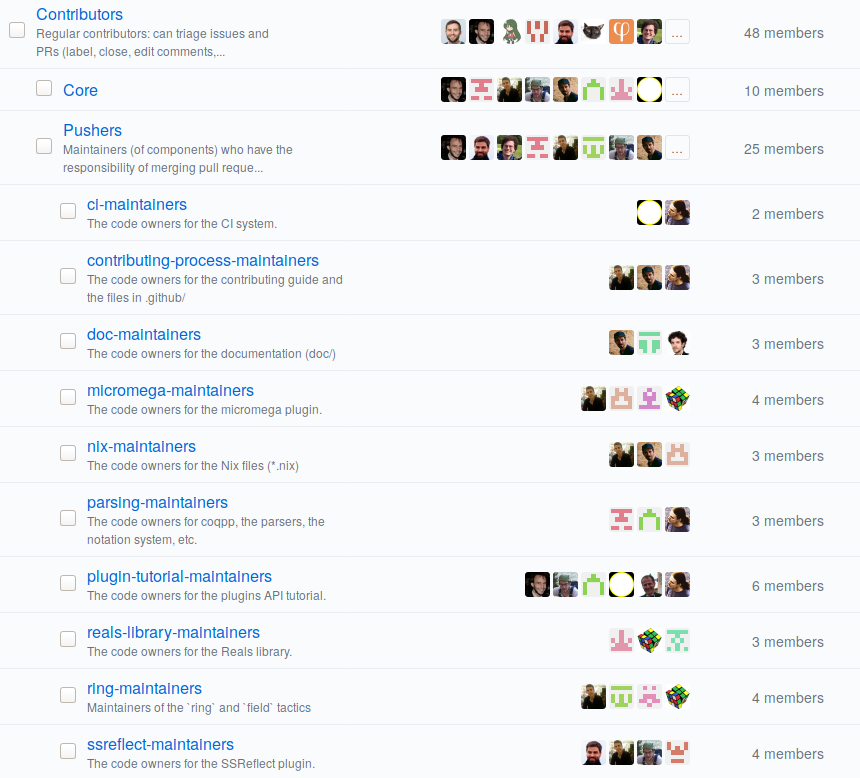
\includegraphics[width=15cm]{maintainer-teams.png}
	\caption{
		The list of teams with access to the Coq repository as of September 11\textsuperscript{th}, 2019.
		The ``Contributors'' team members have write access without the ability to push, to be able to participate to issue and pull request triaging.
		The ``Core'' team reflects who are the administrators of the Coq organization.
		The ``Pushers'' team members have the permission to merge approved pull requests to the master branch.
		The various sub-teams of the ``Pushers'' team are the code owners of various components.
	}
	\label{fig:teams}
\end{figure}

\subsection{Open issues, future work}

\label{sec:open-issues-distributed-merging}

While the merging script is an efficient way of reminding a diversified team of integrators about some criteria that must be satisfied for a pull request to be merged, it also creates a barrier of entry.
Indeed, this script requires some dependencies to be installed, a certain setup of the integrator's local clone of the Coq repository, and that the integrator has a GPG key associated to their git identity.
A way to lower this barrier of entry would be to avoid the integrators to use this script, by allowing them to merge a pull request by issuing a command to the bot.
In fact, I should be able to add this feature soon, because most of the required infrastructure, in particular to check that the person issuing the command belongs to the appropriate team, is already implemented.

Despite the progress that has been made regarding the pull request integration process, it is still not satisfying on several aspects, since it receives regular complaints coming from a few developers.
In particular, they complain that pull request integration is too slow, that reviewers do not always provide good feedback, and sometimes request changes on unsound bases, that there is no process to make discussions converge, and finally that decisions to integrate a pull request can sometimes happen too suddenly, and unpredictably, without time for concerned developers to comment, resulting in an overall unfair process.

Some of these impressions might correspond to actual problems worth addressing, and even when they are just impressions, it is important to be able to understand why developers feel that way.
A first step will therefore be to interview developers to list their complaints, and to gather data to try to back up these complaints.
In particular, it is clear that pull request integration efficiency strongly varies depending on the affected components, and therefore may lead different developers to have different perceptions.

Once issues are more clearly identified, it should be possible to decide what is the best solution to address them: whether it is clearer processes, better tooling, more community involvement, or only conscious efforts from concerned developers.

\section{Conclusion}

In this chapter, I have presented the challenges associated with the adoption of pull requests in the development of Coq.
The experience report from this project confirms what was observed by Dias \emph{et al.}~\cite{dias2016does}: that moving to GitHub alone is not sufficient to attract more contributions.
In fact, for the first few years, mirroring the Coq project on GitHub, and even switching to git, did not impact the development model, or the number of contributors.

However, when the development team decided to take specific steps to attract more contributors, such as organizing workshops, opening a chatroom, improving the developers' documentation, and in particular providing clear contribution guidelines, this was followed by a strong increase in the participation of external contributors.
Some new contributors even participate now to the integration of pull requests.

It is worth noting that this contrasts with the result that will be presented in Chapter~\ref{chap:bug-tracker}: that a simple switch of bug tracker to GitHub had strong effects on both the level of bug tracking activity, and the participation of external contributors.

Besides the impact on the number of contributors, the switch to a pull-based development model was also an opportunity to improve the quality of integrated changes.
I have shown how the introduction of pull request templates with a checklist triggered an increase in the proportion of pull requests including documentation, a changelog entry, and tests.
In particular, the proportion of feature pull requests including a changelog entry increased dramatically.

I have also presented our innovative model for \emph{a priori} compatibility testing, and how it has helped produce more stable releases, where compatibility breaking changes are clearly acknowledged, and migration paths are documented.
